\documentclass[11pt]{article}

\usepackage[a4paper,margin=1in]{geometry}
\usepackage{graphicx}
\usepackage{booktabs}
\usepackage{float}
\usepackage{hyperref}
\usepackage{amsmath}
\usepackage{array}
\usepackage{caption}
\usepackage{fancyhdr}
\usepackage{xcolor}
\usepackage{tikz}

\definecolor{UFBlue}{HTML}{0021A5}
\definecolor{UFOrange}{HTML}{FA4616}
\definecolor{DarkGray}{HTML}{333333}

\hypersetup{colorlinks=true,linkcolor=UFBlue,urlcolor=UFBlue,citecolor=UFBlue}
\setlength{\headheight}{14pt}
\pagestyle{fancy}
\fancyhf{}
\fancyhead[L]{\small\textcolor{UFBlue}{COP5615 --- Distributed Operating Systems Principles}}
\fancyhead[R]{\small\textcolor{DarkGray}{Project 2: Gossip Simulator}}
\fancyfoot[C]{\small\thepage}
\renewcommand{\headrulewidth}{0.5pt}
\setlength{\parindent}{0pt}
\setlength{\parskip}{5pt}

\begin{document}

\begin{titlepage}
\thispagestyle{empty}
\begin{center}
\vspace*{0.35in}
\IfFileExists{uf_horizontal_logo_cropped.png}
  {
\includegraphics[width=2.65in]{uf_horizontal_logo_cropped.png}}
  {\textcolor{UFBlue}{\Large UNIVERSITY OF FLORIDA}}
\vspace{0.65in}

{\Large\bfseries\textcolor{UFBlue}{COP5615 --- DISTRIBUTED OPERATING SYSTEMS PRINCIPLES}\par}
\vspace{0.45in}
{\LARGE\bfseries Project 2\par}
\vspace{0.15in}
{\Huge\bfseries\textcolor{UFBlue}{Bonus: Failure Model}\par}
\vspace{0.25in}
{\color{UFOrange}\rule{4.6in}{1.5pt}}
\vspace{0.45in}

{\large Permanent Connection Failures\par}
\vspace{0.5in}
{\large Pradhyuman Singh Shekhawat\par}
\vspace{0.15in}
{\large October 2026\par}
\vfill
\end{center}
\end{titlepage}

\section{Objective}
The bonus extends the Gossip Simulator with a parameter-controlled
permanent connection-failure model. The experiment investigates how
randomly removing connections affects network connectivity and the
convergence of Gossip and Push-Sum across two topologies.

\section{Implementation}
Let \(p\in[0,1]\) denote the probability that an undirected connection
fails permanently. The failure model first obtains the topology's
undirected edges. Each edge is independently retained with probability
\(1-p\) or removed with probability \(p\). A removed edge is deleted
from both endpoint neighbor lists, ensuring that neither endpoint can
use the failed connection.

Before starting the algorithm, the coordinator checks whether the
remaining graph is connected. If it is disconnected, the trial is
recorded as \texttt{disconnected}; otherwise, the selected algorithm
runs on the surviving graph. This is a permanent topology change for
the duration of a trial, rather than a random decision to drop each
individual message.

\section{Experimental Setup}
The experiments use nine nodes and the \texttt{full} and \texttt{2D}
topologies. Both Gossip and Push-Sum were evaluated at
\(p\in\{0,0.1,0.25,0.5,0.75,1.0\}\), with ten trials per configuration:
\(2\times2\times6\times10=240\) trials in total. Each run used a
5,000 ms convergence timeout.

The CSV file records the status and convergence time of each trial.
Successful convergence, disconnection, timeout, and error are treated
as distinct outcomes. Mean convergence time is calculated only from
successful trials, so it should not be interpreted as the expected
completion time across all trials.

\section{Results}
Table~\ref{tab:results} and Figures~\ref{fig:success}--\ref{fig:disconnected}
are generated from the recorded CSV results. The plots separate the
two topologies into panels to make the Gossip and Push-Sum trends
distinguishable.

\begin{table}[H]
\centering\small
\begin{tabular}{llrrrrr}
\toprule
Algorithm & Topology & $p$ & Success & Disconnected & Timeout & Mean time ($\mu$s) \\
\midrule
Gossip & full & 0 & 10/10 & 0/10 & 0/10 & 28.9 \\
Gossip & full & 0.1 & 10/10 & 0/10 & 0/10 & 28.5 \\
Gossip & full & 0.25 & 9/10 & 0/10 & 1/10 & 44.4 \\
Gossip & full & 0.5 & 7/10 & 0/10 & 3/10 & 102.3 \\
Gossip & full & 0.75 & 1/10 & 5/10 & 4/10 & 128.0 \\
Gossip & full & 1 & 0/10 & 10/10 & 0/10 & -- \\
Gossip & 2D & 0 & 6/10 & 0/10 & 4/10 & 95.5 \\
Gossip & 2D & 0.1 & 3/10 & 1/10 & 6/10 & 95.0 \\
Gossip & 2D & 0.25 & 3/10 & 5/10 & 2/10 & 95.7 \\
Gossip & 2D & 0.5 & 0/10 & 10/10 & 0/10 & -- \\
Gossip & 2D & 0.75 & 0/10 & 10/10 & 0/10 & -- \\
Gossip & 2D & 1 & 0/10 & 10/10 & 0/10 & -- \\
Push-Sum & full & 0 & 10/10 & 0/10 & 0/10 & 1825.6 \\
Push-Sum & full & 0.1 & 10/10 & 0/10 & 0/10 & 1271.9 \\
Push-Sum & full & 0.25 & 10/10 & 0/10 & 0/10 & 1431.4 \\
Push-Sum & full & 0.5 & 10/10 & 0/10 & 0/10 & 1642.3 \\
Push-Sum & full & 0.75 & 4/10 & 6/10 & 0/10 & 3497.8 \\
Push-Sum & full & 1 & 0/10 & 10/10 & 0/10 & -- \\
Push-Sum & 2D & 0 & 10/10 & 0/10 & 0/10 & 2737.8 \\
Push-Sum & 2D & 0.1 & 9/10 & 1/10 & 0/10 & 2899.3 \\
Push-Sum & 2D & 0.25 & 5/10 & 5/10 & 0/10 & 3684.6 \\
Push-Sum & 2D & 0.5 & 2/10 & 8/10 & 0/10 & 5182.5 \\
Push-Sum & 2D & 0.75 & 0/10 & 10/10 & 0/10 & -- \\
Push-Sum & 2D & 1 & 0/10 & 10/10 & 0/10 & -- \\
\bottomrule
\end{tabular}
\caption{Results for ten trials per configuration. Mean convergence time includes successful trials only.}\label{tab:results}
\end{table}

\begin{figure}[H]
\centering
\begin{minipage}{0.48\textwidth}
\centering
\textbf{full topology}\\[2pt]
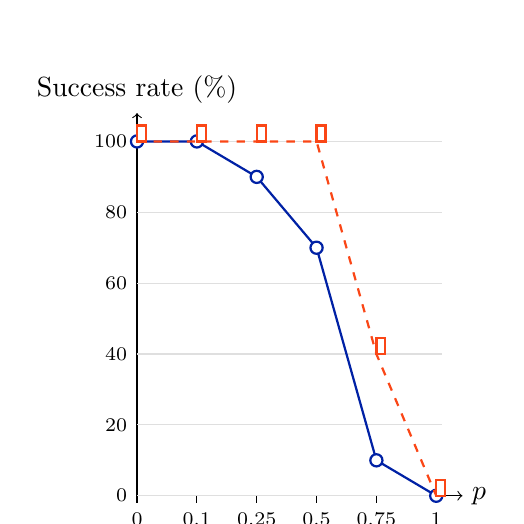
\begin{tikzpicture}[x=0.95cm,y=0.045cm]
\draw[->] (0,0) -- (4.35,0) node[right] {$p$};
\draw[->] (0,0) -- (0,108) node[above,align=center] {Success rate (\%)};
\draw[gray!25] (0,0) -- (4.08,0);
\node[left] at (0,0) {\scriptsize 0};
\draw[gray!25] (0,20) -- (4.08,20);
\node[left] at (0,20) {\scriptsize 20};
\draw[gray!25] (0,40) -- (4.08,40);
\node[left] at (0,40) {\scriptsize 40};
\draw[gray!25] (0,60) -- (4.08,60);
\node[left] at (0,60) {\scriptsize 60};
\draw[gray!25] (0,80) -- (4.08,80);
\node[left] at (0,80) {\scriptsize 80};
\draw[gray!25] (0,100) -- (4.08,100);
\node[left] at (0,100) {\scriptsize 100};
\draw (0.0,0) -- (0.0,-2);
\node[below] at (0.0,-2) {\scriptsize 0};
\draw (0.8,0) -- (0.8,-2);
\node[below] at (0.8,-2) {\scriptsize 0.1};
\draw (1.6,0) -- (1.6,-2);
\node[below] at (1.6,-2) {\scriptsize 0.25};
\draw (2.4,0) -- (2.4,-2);
\node[below] at (2.4,-2) {\scriptsize 0.5};
\draw (3.2,0) -- (3.2,-2);
\node[below] at (3.2,-2) {\scriptsize 0.75};
\draw (4.0,0) -- (4.0,-2);
\node[below] at (4.0,-2) {\scriptsize 1};
\draw[thick,UFBlue,solid] (0.0,100) -- (0.8,100) -- (1.6,90) -- (2.4,70) -- (3.2,10) -- (4.0,0);
\filldraw[fill=white,draw=UFBlue,thick] (0.0,100) circle (2.2pt);
\filldraw[fill=white,draw=UFBlue,thick] (0.8,100) circle (2.2pt);
\filldraw[fill=white,draw=UFBlue,thick] (1.6,90) circle (2.2pt);
\filldraw[fill=white,draw=UFBlue,thick] (2.4,70) circle (2.2pt);
\filldraw[fill=white,draw=UFBlue,thick] (3.2,10) circle (2.2pt);
\filldraw[fill=white,draw=UFBlue,thick] (4.0,0) circle (2.2pt);
\draw[thick,UFOrange,dashed] (0.0,100) -- (0.8,100) -- (1.6,100) -- (2.4,100) -- (3.2,40) -- (4.0,0);
\filldraw[fill=white,draw=UFOrange,thick] (0.0,100) rectangle ++(0.12,4.5);
\filldraw[fill=white,draw=UFOrange,thick] (0.8,100) rectangle ++(0.12,4.5);
\filldraw[fill=white,draw=UFOrange,thick] (1.6,100) rectangle ++(0.12,4.5);
\filldraw[fill=white,draw=UFOrange,thick] (2.4,100) rectangle ++(0.12,4.5);
\filldraw[fill=white,draw=UFOrange,thick] (3.2,40) rectangle ++(0.12,4.5);
\filldraw[fill=white,draw=UFOrange,thick] (4.0,0) rectangle ++(0.12,4.5);
\end{tikzpicture}
\end{minipage}
\hfill
\begin{minipage}{0.48\textwidth}
\centering
\textbf{2D topology}\\[2pt]
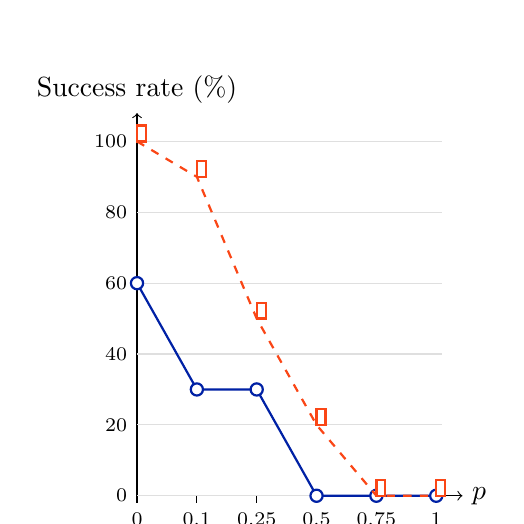
\begin{tikzpicture}[x=0.95cm,y=0.045cm]
\draw[->] (0,0) -- (4.35,0) node[right] {$p$};
\draw[->] (0,0) -- (0,108) node[above,align=center] {Success rate (\%)};
\draw[gray!25] (0,0) -- (4.08,0);
\node[left] at (0,0) {\scriptsize 0};
\draw[gray!25] (0,20) -- (4.08,20);
\node[left] at (0,20) {\scriptsize 20};
\draw[gray!25] (0,40) -- (4.08,40);
\node[left] at (0,40) {\scriptsize 40};
\draw[gray!25] (0,60) -- (4.08,60);
\node[left] at (0,60) {\scriptsize 60};
\draw[gray!25] (0,80) -- (4.08,80);
\node[left] at (0,80) {\scriptsize 80};
\draw[gray!25] (0,100) -- (4.08,100);
\node[left] at (0,100) {\scriptsize 100};
\draw (0.0,0) -- (0.0,-2);
\node[below] at (0.0,-2) {\scriptsize 0};
\draw (0.8,0) -- (0.8,-2);
\node[below] at (0.8,-2) {\scriptsize 0.1};
\draw (1.6,0) -- (1.6,-2);
\node[below] at (1.6,-2) {\scriptsize 0.25};
\draw (2.4,0) -- (2.4,-2);
\node[below] at (2.4,-2) {\scriptsize 0.5};
\draw (3.2,0) -- (3.2,-2);
\node[below] at (3.2,-2) {\scriptsize 0.75};
\draw (4.0,0) -- (4.0,-2);
\node[below] at (4.0,-2) {\scriptsize 1};
\draw[thick,UFBlue,solid] (0.0,60) -- (0.8,30) -- (1.6,30) -- (2.4,0) -- (3.2,0) -- (4.0,0);
\filldraw[fill=white,draw=UFBlue,thick] (0.0,60) circle (2.2pt);
\filldraw[fill=white,draw=UFBlue,thick] (0.8,30) circle (2.2pt);
\filldraw[fill=white,draw=UFBlue,thick] (1.6,30) circle (2.2pt);
\filldraw[fill=white,draw=UFBlue,thick] (2.4,0) circle (2.2pt);
\filldraw[fill=white,draw=UFBlue,thick] (3.2,0) circle (2.2pt);
\filldraw[fill=white,draw=UFBlue,thick] (4.0,0) circle (2.2pt);
\draw[thick,UFOrange,dashed] (0.0,100) -- (0.8,90) -- (1.6,50) -- (2.4,20) -- (3.2,0) -- (4.0,0);
\filldraw[fill=white,draw=UFOrange,thick] (0.0,100) rectangle ++(0.12,4.5);
\filldraw[fill=white,draw=UFOrange,thick] (0.8,90) rectangle ++(0.12,4.5);
\filldraw[fill=white,draw=UFOrange,thick] (1.6,50) rectangle ++(0.12,4.5);
\filldraw[fill=white,draw=UFOrange,thick] (2.4,20) rectangle ++(0.12,4.5);
\filldraw[fill=white,draw=UFOrange,thick] (3.2,0) rectangle ++(0.12,4.5);
\filldraw[fill=white,draw=UFOrange,thick] (4.0,0) rectangle ++(0.12,4.5);
\end{tikzpicture}
\end{minipage}
\caption{Successful convergence rate as connection-failure probability increases. Each point summarizes ten trials.}\label{fig:success}
\end{figure}

\begin{figure}[H]
\centering
\begin{minipage}{0.48\textwidth}
\centering
\textbf{full topology}\\[2pt]
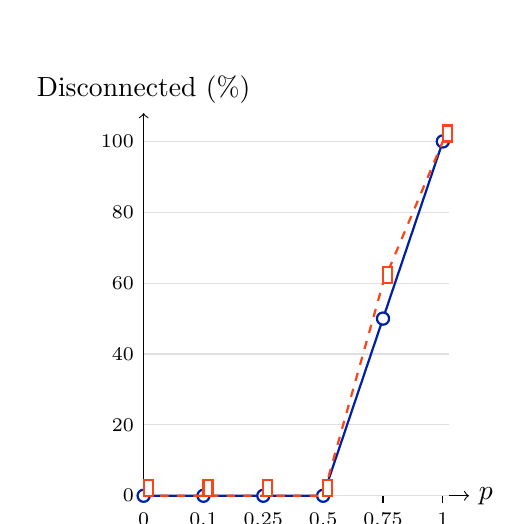
\begin{tikzpicture}[x=0.95cm,y=0.045cm]
\draw[->] (0,0) -- (4.35,0) node[right] {$p$};
\draw[->] (0,0) -- (0,108) node[above,align=center] {Disconnected (\%)};
\draw[gray!25] (0,0) -- (4.08,0);
\node[left] at (0,0) {\scriptsize 0};
\draw[gray!25] (0,20) -- (4.08,20);
\node[left] at (0,20) {\scriptsize 20};
\draw[gray!25] (0,40) -- (4.08,40);
\node[left] at (0,40) {\scriptsize 40};
\draw[gray!25] (0,60) -- (4.08,60);
\node[left] at (0,60) {\scriptsize 60};
\draw[gray!25] (0,80) -- (4.08,80);
\node[left] at (0,80) {\scriptsize 80};
\draw[gray!25] (0,100) -- (4.08,100);
\node[left] at (0,100) {\scriptsize 100};
\draw (0.0,0) -- (0.0,-2);
\node[below] at (0.0,-2) {\scriptsize 0};
\draw (0.8,0) -- (0.8,-2);
\node[below] at (0.8,-2) {\scriptsize 0.1};
\draw (1.6,0) -- (1.6,-2);
\node[below] at (1.6,-2) {\scriptsize 0.25};
\draw (2.4,0) -- (2.4,-2);
\node[below] at (2.4,-2) {\scriptsize 0.5};
\draw (3.2,0) -- (3.2,-2);
\node[below] at (3.2,-2) {\scriptsize 0.75};
\draw (4.0,0) -- (4.0,-2);
\node[below] at (4.0,-2) {\scriptsize 1};
\draw[thick,UFBlue,solid] (0.0,0) -- (0.8,0) -- (1.6,0) -- (2.4,0) -- (3.2,50) -- (4.0,100);
\filldraw[fill=white,draw=UFBlue,thick] (0.0,0) circle (2.2pt);
\filldraw[fill=white,draw=UFBlue,thick] (0.8,0) circle (2.2pt);
\filldraw[fill=white,draw=UFBlue,thick] (1.6,0) circle (2.2pt);
\filldraw[fill=white,draw=UFBlue,thick] (2.4,0) circle (2.2pt);
\filldraw[fill=white,draw=UFBlue,thick] (3.2,50) circle (2.2pt);
\filldraw[fill=white,draw=UFBlue,thick] (4.0,100) circle (2.2pt);
\draw[thick,UFOrange,dashed] (0.0,0) -- (0.8,0) -- (1.6,0) -- (2.4,0) -- (3.2,60) -- (4.0,100);
\filldraw[fill=white,draw=UFOrange,thick] (0.0,0) rectangle ++(0.12,4.5);
\filldraw[fill=white,draw=UFOrange,thick] (0.8,0) rectangle ++(0.12,4.5);
\filldraw[fill=white,draw=UFOrange,thick] (1.6,0) rectangle ++(0.12,4.5);
\filldraw[fill=white,draw=UFOrange,thick] (2.4,0) rectangle ++(0.12,4.5);
\filldraw[fill=white,draw=UFOrange,thick] (3.2,60) rectangle ++(0.12,4.5);
\filldraw[fill=white,draw=UFOrange,thick] (4.0,100) rectangle ++(0.12,4.5);
\end{tikzpicture}
\end{minipage}
\hfill
\begin{minipage}{0.48\textwidth}
\centering
\textbf{2D topology}\\[2pt]
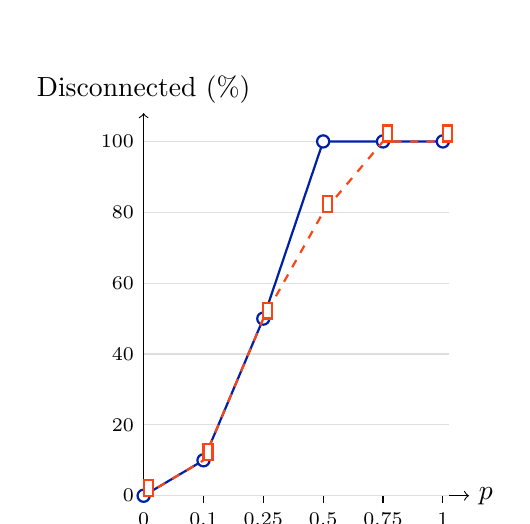
\begin{tikzpicture}[x=0.95cm,y=0.045cm]
\draw[->] (0,0) -- (4.35,0) node[right] {$p$};
\draw[->] (0,0) -- (0,108) node[above,align=center] {Disconnected (\%)};
\draw[gray!25] (0,0) -- (4.08,0);
\node[left] at (0,0) {\scriptsize 0};
\draw[gray!25] (0,20) -- (4.08,20);
\node[left] at (0,20) {\scriptsize 20};
\draw[gray!25] (0,40) -- (4.08,40);
\node[left] at (0,40) {\scriptsize 40};
\draw[gray!25] (0,60) -- (4.08,60);
\node[left] at (0,60) {\scriptsize 60};
\draw[gray!25] (0,80) -- (4.08,80);
\node[left] at (0,80) {\scriptsize 80};
\draw[gray!25] (0,100) -- (4.08,100);
\node[left] at (0,100) {\scriptsize 100};
\draw (0.0,0) -- (0.0,-2);
\node[below] at (0.0,-2) {\scriptsize 0};
\draw (0.8,0) -- (0.8,-2);
\node[below] at (0.8,-2) {\scriptsize 0.1};
\draw (1.6,0) -- (1.6,-2);
\node[below] at (1.6,-2) {\scriptsize 0.25};
\draw (2.4,0) -- (2.4,-2);
\node[below] at (2.4,-2) {\scriptsize 0.5};
\draw (3.2,0) -- (3.2,-2);
\node[below] at (3.2,-2) {\scriptsize 0.75};
\draw (4.0,0) -- (4.0,-2);
\node[below] at (4.0,-2) {\scriptsize 1};
\draw[thick,UFBlue,solid] (0.0,0) -- (0.8,10) -- (1.6,50) -- (2.4,100) -- (3.2,100) -- (4.0,100);
\filldraw[fill=white,draw=UFBlue,thick] (0.0,0) circle (2.2pt);
\filldraw[fill=white,draw=UFBlue,thick] (0.8,10) circle (2.2pt);
\filldraw[fill=white,draw=UFBlue,thick] (1.6,50) circle (2.2pt);
\filldraw[fill=white,draw=UFBlue,thick] (2.4,100) circle (2.2pt);
\filldraw[fill=white,draw=UFBlue,thick] (3.2,100) circle (2.2pt);
\filldraw[fill=white,draw=UFBlue,thick] (4.0,100) circle (2.2pt);
\draw[thick,UFOrange,dashed] (0.0,0) -- (0.8,10) -- (1.6,50) -- (2.4,80) -- (3.2,100) -- (4.0,100);
\filldraw[fill=white,draw=UFOrange,thick] (0.0,0) rectangle ++(0.12,4.5);
\filldraw[fill=white,draw=UFOrange,thick] (0.8,10) rectangle ++(0.12,4.5);
\filldraw[fill=white,draw=UFOrange,thick] (1.6,50) rectangle ++(0.12,4.5);
\filldraw[fill=white,draw=UFOrange,thick] (2.4,80) rectangle ++(0.12,4.5);
\filldraw[fill=white,draw=UFOrange,thick] (3.2,100) rectangle ++(0.12,4.5);
\filldraw[fill=white,draw=UFOrange,thick] (4.0,100) rectangle ++(0.12,4.5);
\end{tikzpicture}
\end{minipage}
\caption{Fraction of trials whose remaining graph was disconnected. Each point summarizes ten trials.}\label{fig:disconnected}
\end{figure}



\section{Observations}
The results show that topology affects tolerance to permanent
connection failures. In the full topology, Push-Sum converged in all
ten trials at each tested probability from \(p=0\) through \(p=0.5\).
At \(p=0.75\), it converged in four of ten trials. In the 2D topology,
Push-Sum success decreased from ten of ten trials at \(p=0\), to five
of ten at \(p=0.25\), and two of ten at \(p=0.5\).

Gossip also showed a sharper decline in the 2D topology: it converged
in three of ten trials at \(p=0.1\) and \(p=0.25\), and none at
\(p\geq0.5\). For the full topology, Gossip converged in all ten
trials at \(p=0\) and \(p=0.1\), and seven of ten at \(p=0.5\).

These observations are consistent with the full topology having more
alternative paths between nodes. Removing edges from a grid can more
readily disconnect it or leave a graph on which the algorithm fails to
finish before the timeout. The experiment supports this conclusion for
the tested graph size, parameter values, and random trials; it does
not establish a universal ranking for every network size.

\section{Limitations}
The experiments use ten random trials per configuration, so measured
rates can vary with the sampled failed edges. A timeout means that
the algorithm did not report convergence within five seconds; it does
not prove that convergence is impossible. A disconnected graph is
reported separately because the coordinator rejects it before the
algorithm runs. This experiment models permanent connection failures;
it does not implement node crashes or temporary connection recovery.

\section{Conclusion}
The bonus implements a parameter-controlled permanent undirected
connection-failure model, tests its effects on Gossip and Push-Sum,
and records the outcomes over 240 trials. The observed results show
that the full topology generally retains successful convergence at
higher tested failure probabilities than the 2D topology. The
conclusion is limited to the tested configurations and trial counts.

\end{document}
